% !Mode:: "TeX:UTF-8"

\documentclass[12pt,oneside]{book}

\newlength{\textpt}
\setlength{\textpt}{12pt}
    
\newcommand{\flypage}[1]{\begin{titlepage}\begin{center}\vspace*{\stretch{1}}#1\vspace*{\stretch{1}}\end{center}\end{titlepage}}
    
%========基本必备的宏包========%
\RequirePackage{calc,float,moresize}
%\RequirePackage[onehalfspacing]{setspace}
\linespread{1.5}
%1.3 onehalfspacing
%试卷或需要文字紧凑的
%1.6 doublespacing

%===========加入目录 某章或某节=====%
\makeatletter

\newcommand{\addchtoc}[1]{
        \cleardoublepage
        \phantomsection
        \addcontentsline{toc}{chapter}{#1}}

\newcommand{\addsectoc}[1]{
        \phantomsection
        \addcontentsline{toc}{section}{#1}}

%===========全文基本格式==========%
\setlength{\parskip}{1.6ex plus 0.2ex minus 0.2ex}   %段落間距
\setlength{\parindent}{\textpt * \real{2}}

%=========页面设置=========%
\RequirePackage[a4paper, %a4paper size 297:210 mm
  bindingoffset=10mm,%裝訂線
  top=35mm,  %上邊距 包括頁眉
  bottom=30mm,%下邊距 包括頁腳
  inner=10mm,  %左邊距or inner
  outer=10mm,  %右邊距or  outer
  headheight=10mm,%頁眉
  headsep=15mm,%
  footskip=15mm,%
  marginparsep=10pt, %旁註與正文間距
  marginparwidth=6em,includemp=true% 旁註寬度計入width%旁註寬度
  ]{geometry}

%color
\RequirePackage[table,svgnames]{xcolor}

%================字體================%
%设置数学字体
\RequirePackage{amssymb,amsmath}
\RequirePackage{stmaryrd}
\everymath{\displaystyle}

\RequirePackage{fontspec}
%設置英文字體
\setmainfont[Mapping=tex-text]{DejaVu Serif}
\setsansfont[Mapping=tex-text]{DejaVu Sans}
\setmonofont[Mapping=tex-text]{DejaVu Sans Mono}


%中文環境
\RequirePackage[]{xeCJK}
\xeCJKsetup{PunctStyle=plain}
\xeCJKDeclareSubCJKBlock{LIUSHISIGUA}{ "4DC0 -> "4DFF}
\setCJKmainfont[FallBack=DejaVu Serif, ItalicFont=KaiTi,LIUSHISIGUA=DejaVu Sans]{Source Han Serif CN}
\setCJKsansfont[FallBack=DejaVu Sans]{Source Han Sans CN}
\setCJKmonofont[FallBack=DejaVu Sans Mono]{KaiTi}


%%===============中文化=========%
\renewcommand\contentsname{目~录}
\renewcommand\listfigurename{插图目录}
\renewcommand\listtablename{表格目录}
\renewcommand\bibname{参~考~文~献}
\renewcommand\indexname{索~引}
\renewcommand\figurename{图}
\renewcommand\tablename{表}
\renewcommand\partname{部分}
\renewcommand\appendixname{附录}
\renewcommand{\today}{\number\year{}年\number\month{}月\number\day{}日}


%=======页眉页脚格式=========%
\RequirePackage{fancyhdr}   %頁眉頁腳
\RequirePackage{zhnumber}  %计数器中文化
\pagestyle{fancy}
\renewcommand{\sectionmark}[1]
{\markright{第\zhnumber{\arabic{section}}节~~#1}{}}

\fancypagestyle{plain}{%
    \fancyhf{}
    \renewcommand{\headrulewidth}{0pt}
    \renewcommand{\footrulewidth}{0pt}
    \fancyhf[HR]{\ttfamily \footnotesize \rightmark }
    \fancyhf[FR]{\thepage}}
\pagestyle{plain}


%=========章節標題設計=========%
\RequirePackage{titlesec}
%修改part
\titleformat{\part}{\huge\sffamily}{}{0em}{}
%修改chapter
\titleformat{\chapter}{\LARGE\sffamily}{}{0em}{}
%修改section
\titleformat{\section}{\Large\sffamily}{}{0em}{}
%修改subsection
\titleformat{\subsection}{\large\sffamily}{}{0em}{}
%修改subsubsection
\titleformat{\subsubsection}{\normalsize\sffamily}{}{0em}{}


%================目录===============%
%toc label to contents space   dynamic adjust
\RequirePackage{tocloft}%
\renewcommand{\numberline}[1]{%
  \@cftbsnum #1\@cftasnum~\@cftasnumb%
}

%==============超鏈接===============%
\RequirePackage[colorlinks=true,linkcolor=blue,citecolor=blue]{hyperref} %設置書簽和目錄鏈接等
\newcommand{\hlabel}[1]{\phantomsection \label{#1}}%某一小段的引用


%=================文字強調=========%
\RequirePackage{xeCJKfntef}

\let\oldemph\emph % Save emph in oldemph
\renewcommand{\emph}[1]{\textcolor{red}{#1}}  

%==================插入圖片=======%
\RequirePackage{wrapfig}
\RequirePackage{graphicx}
\graphicspath{{figures/}}
%change the caption style a little like 1-1
\renewcommand{\thefigure}{\arabic{chapter}-\arabic{figure}}

%插入代码
\RequirePackage{fancyvrb} 
\fvset{frame=lines,tabsize=4 ,baselinestretch=1.8, fontsize=\footnotesize}


%==========其他宏包===========%
\RequirePackage{tikz} 
\usetikzlibrary{calc}

%========脚注=========%
\newcommand*\circled[1]{
\tikz[baseline=(char.base)]
\node[shape=circle,draw,inner sep=0.4pt,minimum size=4pt] (char) {#1};}

\newcommand*\circledarabic[1]{\circled{\arabic{#1}}}

\RequirePackage{perpage} %the perpage package
\MakePerPage{footnote} %the perpage package command

\renewcommand*{\thefootnote}{\protect\circledarabic{footnote}}


\renewcommand\@makefntext[1]{\vspace{5pt}\noindent
\makebox[20pt][c]{\fontsize{10pt}{12pt}\@thefnmark}
\fontsize{10pt}{12pt}\selectfont #1}

\setlength{\skip\footins}{20pt plus 10pt}
%main body 与脚注之间的距离

\RequirePackage{indentfirst} 

% hr
\newcommand\hr{\par\noindent\hrule}

%重新定义quotation
\AtBeginEnvironment{quotation}{\ttfamily}

\makeatother

\title{冶文房}
\author{Wander}
\hypersetup{
  pdfkeywords={},
  pdfsubject={制作者邮箱:a358003542@outlook.com},
  pdfcreator={Wander}}
  
\newcommand{\bookcover}[1]{\tikz[remember picture,overlay]{\node[inner sep=0] at (current page.center)
{\includegraphics[width=\paperwidth,height=\paperheight]{#1}}}} 
 

  
\begin{document}
\frontmatter 

\thispagestyle{empty}

\bookcover{book_cover.png}

\cleardoublepage



\addchtoc{前言}
\chapter*{前言}
冶炼文字,以成此集。


\addchtoc{目录}
\setcounter{tocdepth}{2}    
\tableofcontents



\mainmatter

\part{十三世纪之前}
\chapter{黄帝内经关于养生之道的讨论}
\hr
[黄帝]乃问于天师曰:余闻上古之人,春秋皆度百岁,而动作不衰;今时之人,年半百而动作皆衰者,时世异耶,人将失之耶?

歧伯对曰:上古之人,其知道者,法于阴阳,和于术数,食饮有节,起居有常,不妄作劳,故能形与神俱,而尽终其天年,度百岁乃去。今时之人不然也,以酒为浆,以妄为常,醉以入房,以欲竭其精,以耗散其真,不知持满,不时御神,务快其心,逆于生乐,起居无节,故半百而衰也。夫上古圣人之教下也,皆谓之虚邪贼风,避之有时,恬惔虚无,真气从之,精神内守,病安从来。是以志闲而少欲,心安而不惧,形劳而不倦,气从以顺,各从其欲,皆得所愿。故美其食,任其服,乐其俗,高下不相慕,其民故曰朴。是以嗜欲不能劳其目,淫邪不能惑其心,愚智贤不肖不惧于物,故合于道。所以能年皆度百岁而动作不衰者,以其德全不危也。
\hr

 
黄帝曾向天师岐伯请教道:我听说上古时代的人们,都能够年过百岁,行动起来却不显衰老;而现在的人,年过半百,行动就已经显得很衰老了。这是由于时代不同了呢?还是由于人们违背了养生之道呢?

岐伯答道:上古时代的人,大都懂得养生之道,效法于天地阴阳变化,和谐于身心养生之术,饮食有节制,起居有规律,劳作适度,所以能够使身体与精神协调一致,从而尽享天年,度过百岁才离开人世。现在的人却不是这样,把酒当做果浆来喝,把任意妄为当作生活的常态,酒醉之后还强行房事,在放纵淫欲中使自己的精气枯竭,真元耗散,不懂得保持精气的盈满,不知适时御凝己神,只求一时快意开心,如此违逆了生活真正的乐趣,起居没有规律,故年半百就衰老了。上古时代圣人的教诲,都是这样说的:要适时回避四季不正的虚邪贼风,思想上恬淡虚无,体内真气随从其中,精神持守其内,疾病又从那里来呢。如此志闲淡而少欲,心安宁而无惧,形劳作而不疲倦,真气随从而调顺,每个人欲望和愿望都很容易得到满足。如此吃什么都很香甜,穿什么都很舒服,快乐地享受他们的习俗,彼此也不羡慕地位高低,民风可称纯朴。如此嗜好欲望颇深之物不能劳累其眼,淫乱邪恶之物不能惑乱其心,不论愚笨还是聪明,贤能或者不才之人都不惧怕物欲之物,而合于养生之道。所以他们能年过百岁而行动不衰,就是因为他们[如上]德行全备而无偏颇的缘故啊。


\part{十三世纪}

\part{十四世纪}

\part{十五世纪}


\part{十六世纪}

\part{十七世纪}

\part{十八世纪}

\part{十九世纪}

\part{二十世纪}

\part{二十一世纪}
\chapter{二十一世纪前期对世界各地葬礼的观察}
\begin{Verbatim}
原文: 《From Here to Eternity》 by Caitlin Doughty 2017. 

译文: 《好好告别:世界葬礼观察手记》 by 崔倩倩 2022.
\end{Verbatim}


\hr
早在2000多年前,古希腊历史学家希罗多德就写过两种文化对彼此的丧葬传统感到震惊的情形,可谓历史上对此现象最早的记录之一。在他的描述中,波斯帝国的统治者召集了一些希腊人到他面前。希腊人有火化遗体的传统,国王便问道:“什么样的奖赏能让你们吃掉父亲的遗体?”这个问题让希腊人惊慌不已,连连解释无论多么丰厚的赏赐都不足以把自己变成食人族。第二天,国王召集了因食用遗体而闻名的卡拉提亚人。国王问他们:“什么样的奖赏能让你们焚烧父亲的遗体?”卡拉提亚人表示这种行径“太可怕了”,请求国王不要再提及此事。
\hr

\section{美国科罗拉多州的克雷斯通镇}
\hr
8月的一个午后,我收到一封期待许久的来信:

凯特琳:

我们社区重要的一员劳拉今早离开了我们。她有心脏病史,刚刚过完75岁生日。不知道你现在身在何处,但欢迎你加入我们。

史蒂芬妮

劳拉的死完全出人意料。周日傍晚,她还在当地的音乐节上纵情起舞,周一一早就被发现倒在厨房的地板上没有了呼吸。火化仪式定在周四上午举行,届时她的家人都会出席,我也会在场。

...

劳拉的家人用布制的担架抬着劳拉穿过一片黑眼花,来到火葬用的火化台旁。一记嘹亮的锣声响彻天空。我沿着停车场旁的沙石小路向前走,一名笑容满面的志愿者递给我一捆新鲜的杜松枝。

劳拉平躺在一块金属炉箅\footnote{bì,蒸锅中的竹屉。}上,左侧和右侧各有一面光滑的白色水泥壁,上方则是一望无际的科罗拉多苍穹。我在这里见过两次空空如也的火化台,但这一次,遗体的出现令我理智、清晰地认识到这种仪式的目的。凭吊的人一个接一个地走上前来,把手中的杜松枝放到劳拉身上。作为唯一不认识劳拉的人,我有些犹豫——我管这个叫葬礼尴尬症。但我既不能一直把杜松枝拿在手里(太明显了),又不能放进背包(太没品了),于是我只好上前把枝条放在遗体上。

接下来,劳拉的家人(包括一个八九岁的小男孩)用矮松木的松枝和云杉原木把柴堆围起来。这两种木材越烧密度越高,所以通常是火化的首选。劳拉的伴侣和她已经成年的儿子手持火把站在角落里。随着信号出现,他们一起走向劳拉,将柴堆点燃。此时,太阳刚好从地平线上升起。

当火焰开始吞噬劳拉的身体时,白色的浓烟像小型旋风似的旋转上升,然后逐渐消失在清晨的天空中。

火化的味道让我想起爱德华·阿比作品中的一段描述:

\begin{quotation}
火焰。在我看来,杜松枝燃烧时发出的香味是世界上最甜美的,我怀疑但丁笔下的天堂都没有能与此媲美的熏香。就像雨后灌木丛的味道,只需闻一下,就能引发魔法般的通感:那是美妙的音乐,那是美国西部的广袤、光明、澄澈和神秘。希望火焰永远燃烧下去。
\end{quotation}

几分钟之后,螺旋状的浓烟不见了踪影,取而代之的是明亮的红色火焰。火焰攒足了能量,足足蹿到6英尺高。参加葬礼的一共有130人,他们全围绕在火化台旁,无声地看着眼前的一切。唯一的声响来自树枝断裂时的“噼啪”声,仿佛劳拉的每一段记忆都随着声响飘散在晨空中。

在科罗拉多州的克雷斯通进行的这种火葬仪式已有上万年的历史。古希腊人、古罗马人及印度教徒,都因使用最朴实的秘术——火——来消除肉体和净化灵魂而闻名于世。但火葬本身还可以追溯到更古老的时期。

20世纪60年代,一名年轻的地质学家在澳大利亚内陆发现了一具火化过的成年女性遗骸。根据他的预测,这具遗骸距今已有20000年。事实上,后续研究表明这名女性应该生活在42000年前,比原住民到达澳大利亚的推测时间还要早22000年。她应该是居住在布满植被的山坡上,和一群巨型生物(袋鼠、袋熊以及其他尺寸超常的啮齿类动物)为伴,以鱼肉、植物的种子和巨型鸸鹋\footnote{ér miáo,鸟纲,鸵鸟目,鸸鹋科。}的蛋为食。她死后,族人便把她(现在被称为“芒戈女士”)火化。没有焚烧完全的遗骨将被捣碎并进行二次火化。最后,族人用红色泥土把遗骸包裹起来埋在地下,一晃就是42000年。

...

美国其他地方也一样:同样规模的小镇,同样悲伤的人群,同样的露天火化台。但这显然不是事实。克雷斯通其实是美国,也是西方世界中唯一以社区为基础来实施露天火化的地方。

这种令人心潮澎湃的火化方式并非一直存在于克雷斯通。...“我们执着于用火化台进行露天火葬。”史蒂芬妮解释道,...

和史蒂芬妮一起工作的还有保罗·克鲁本伯格。他也很讨人喜欢,有着一口厚重的荷兰口音。他们二人带着火化台四处奔走,直接在别人家里进行火化。为了不让镇政府发现,两个人练就了一身速战速决的本领。就这样,他们用这套可移动设备完成了七场火葬。

“我们只要在你家院子的角落里把设备组装好就能开工。”保罗说道。

他们这套可移动火化台设备技术含量并不高,主要用煤渣砖制成,外加一个炉箅。每次火化时产生的高温都会让炉箅弯曲变形。“我们不得不开车碾过去,直接把它轧平。”史蒂芬妮说,“现在看来,我们当时确实很疯狂。”她边说边笑,并不觉得以前的做法有何不妥。

2006年,二人决定寻找一处固定场所来执行露天火葬。克雷斯通堪称完美之选:地理位置足够偏远,距离丹佛市中心约四个小时车程,全镇人口只有137人(周边地区人口1400人)。这种边缘性让克雷斯通具备了一种“老子的事儿政府最好别插手”的自由派气质,大麻和妓院在这里都是合法的(并不是说已经开了好几家妓院,只是说可以有)。

克雷斯通吸引了形形色色的“朝圣者”,人们从世界各地来到这里寻找精神家园。当地的天然食品店里贴着各种各样的广告宣传单:气功班、影子智慧班、面向儿童的“潜能开发”灵修班、北非民族舞蹈班,还有什么“魔法森林圣集会”。克雷斯通的本地居民不乏嬉皮士和信托自由儿\footnote{指来自富裕家庭的年轻人。},但大部分都是严肃的终身信徒。这里有佛教徒、苏菲主义者、卡迈尔修女等。刚刚过世的劳拉就是印度哲学家室利·阿罗频多的忠实追随者。

史蒂芬妮和保罗首次申请火葬固定用地时,就遭到了多个业主的反对。“他们是一帮烟民,就这德行。”保罗告诉我。这些业主义正词严地警告他们“别打我地盘的主意”。在史蒂芬妮看来,他们就是一群“守财奴”,根本不在乎二人提供的无林火风险、无异味、无水银或其他有毒物的证据。这些烟民集体给镇政府和环保局写信抗议。

为了抗争,史蒂芬妮和保罗把自己的业务进行了合法化。他们成立了一个名为“克雷斯通临终计划”的非营利机构,一刻不停地收集了400多个签名(相当于周边人口的1/3)。他们把法务文件、科学检测报告等材料通通收集起来,装订成一本厚厚的资料册。他们甚至走访了当地每一户居民,认真倾听大家的担心和顾虑。

一开始,他们遭到了人们的严重抵触。在一次反对露天火葬的集会上,有人叫他们“邻里互助火化二人组”。当史蒂芬妮和保罗提议(其实是个玩笑)在当地游行活动中使用卡通气模进行宣传时,有一家人走过来抗议说这种行为“简直是大不敬”,因为气模上带有火焰形状的纸质装饰品。

“镇上的居民甚至担心露天火葬会导致交通堵塞。”史蒂芬妮说道,“要知道在克雷斯通,一条街上同时出现6辆车都能被看作交通堵塞。”

保罗解释道:“这是因为人们充满了恐惧。‘这会不会造成空气污染?’‘你不觉得这很变态吗?’‘一想到与死有关的东西,我就害怕。’你必须保持耐心,仔细倾听他们的想法和需求。”

哪怕面临诸多法律困境,史蒂芬妮和保罗也没有退缩,因为他们坚信露天火葬能够启发整个社区(一些居民因为自己有机会被露天火葬而激动不已,要求史蒂芬妮和保罗把设备组装在自家的停车道上)。“如今,有多少人能提供真正让别人产生共鸣的服务?”史蒂芬妮说道,“我只做能唤起心灵共鸣的事,不然就不做。”

二人终于给自己的火化台找到了一个稳定的家。那是小镇外的一处空地,距离主路几百码远。这块土地是禅宗团体“龙山庙”捐赠给他们的。史蒂芬妮和保罗毫不遮掩地把火化台放在外面。当你沿着这条主路驶向克雷斯通时,你就会看到一个印有火焰图案的金属标志,上面写着“火化台”三个字。这个标志出自当地一位种土豆的农民之手(这个人同时兼任验尸官),可以说是一个明显的地标了。

火化台搭建在一片沙地之上,四周环绕着一片竹林。竹子的枝条形态各异,好似书法的笔画。目前,这里已经火化了50多人,包括把他们称为“邻里互助火化二人组”的那个人,他在临终前改变了自己的看法(反转无误)。

在为劳拉举行火葬的3天前,克雷斯通临终计划的志愿者来到她家帮忙。他们和劳拉的友人一起打理遗体,帮他们用低温毯裹好遗体以防腐化。他们还给劳拉穿上由天然面料制成的寿衣——化纤面料不适合用在火化台火葬中,比如涤纶。

克雷斯通临终计划会协助死者家属进行所有的葬礼后勤工作,但不为其提供资金支持。死者家属也可以选择露天火葬之外的火化方式:传统土葬(遗体经过防腐),自然土葬(没有墓穴或遗体不经过防腐),去几个镇子之外的火葬场进行火化。不管选择哪一种,志愿者都会协助家属进行相关的后勤工作。保罗把最后一种称为“商业火化”。

史蒂芬妮抗议道:“保罗,你应该叫它‘传统火化’。”

“不不,”我争辩道,“‘商业火化’这个称呼很贴切。”

克雷斯通让身为殡葬业专业人员的我备受鼓舞——这也是我多次来到这里的原因,但也让我感到些许(近乎嫉妒的)忧伤。这里的人们拥有一个庄严的火化台,就在浩瀚苍穹之下,我却只能把家人送到郊区厂房里那个又脏又吵的火葬场。如果我自己的殡仪馆能有一处如此壮观的火化场所,我发誓会请一个迪吉里杜管乐手在现场演奏。

以火化炉作为主要设备的工业火化首先出现在19世纪末期的欧洲。1869年,一群医学专家聚集在意大利佛罗伦萨,宣称土葬存在卫生问题,应该用火化取而代之。几乎是与此同时,一股提倡火化的风潮也席卷了美国,领头人是奥克塔维厄斯·B.弗洛汀汉姆牧师,他认为化作一堆“白色灰烬”的遗体比“高度腐烂”的遗体要好得多。

约瑟夫·亨利·路易斯·查尔斯·德·帕尔姆男爵是第一个在美国经历“科学的现代化”火葬的人。这名男爵是一位身无分文的奥地利落魄贵族,死于1876年5月。用《纽约论坛报》的话来说,“他主要是因为变成了一具尸体而出名”。

火化安排在当年12月,也就是他死去的六个月之后。在这半年里,他的遗体被注入砒霜以防腐烂。当砒霜逐渐失效,不足以抵抗大自然力量的时候,当地的一个殡葬人直接把器官从他体内拽出来,再用黏土和石炭酸的混合物涂满他的全身。在从纽约开往宾夕法尼亚州(火葬场所在地)的火车上,这具已然木乃伊化的尸体还在行李车厢中消失了一段时间。历史学家斯蒂芬·普罗特劳称这段插曲为“令人毛骨悚然的捉迷藏”。

这场具有划时代意义的火化在宾州的一处火葬场进行。这个火葬场由私人诊所改造而成,主要设备是一个火炉,炉箅下方装满了用作燃料的煤块。这样一来,火焰不用接触尸体,光凭高温就能让尸体“分崩离析”。尽管医学专家们一再强调这场火化是“一次严格遵循科学和卫生原理的实验”,德·帕尔姆男爵的遗体还是被撒上香料,安放在铺满了玫瑰、棕榈枝、报春花和松树枝的灵床上。当遗体刚被放入火炉时,观察人员称自己闻到了一股独特的烤人肉味,但很快这个味道就被花朵和香料的芬芳掩盖住了。一个小时之后,德·帕尔姆男爵的遗体上笼罩了一层闪闪发光的玫瑰色薄雾。接着,这层光芒逐渐转变为金色,最终变成了透明的亮红色。遗体就这样烧了两个半小时,直到从白骨化作灰烬。现场的记者和评论员后来在报道中写道,这次实验性火化“第一次实现了把人放在烤箱中进行安全、无味的烘烤”。

从那之后,火化设备变得越发庞大,运转速度越来越快,效率越来越高。大约150年之后,火葬的受欢迎程度达到了历史新高(美国2017年的火葬人数可能超过土葬人数,这在历史上还是头一遭)。但是,火葬的仪式和美学还是老样子。我们的火化设备还在使用19世纪70年代发明出来的款式——用钢铁、水泥和砖块建成的,重达24000磅的庞然大物。这些“怪物”每个月都要消耗上千美元的天然气,向大气中排放大量的二氧化碳、烟尘、二氧化硫,以及毒素含量极高的水银(主要来自遗体内的填充物)。

大城市里的火葬场大多存在于郊外工业区中不起眼的厂房里。...有的火葬场就位于墓地,...

有些火葬场把自己打造成“为生命喝彩”型或“火葬纪念堂”型机构。在那里,死者的亲朋好友聚集在空调屋里,透过玻璃窗目送遗体消失在火化炉的金属门后。火化机则躲藏在墙体后方,这样就不会被来宾看到,虽然它们和你在其他火葬场里见到的工业用火化炉没什么区别。这种伪装让还活着的人越发远离死亡这一事实,也越发远离火化方式笨重陈旧、污染环境这一真相。如果想让死去的母亲享受到“火葬纪念堂”型机构提供的优等待遇,你至少要花上5000美元。

我并没有说选择露天火葬就能解决这些问题。在印度、尼泊尔等将露天火葬作为主要殡葬方式的国家,每年的火化量高达百万场,耗费近5000万棵树,并释放出大量的黑碳气溶胶。黑碳气溶胶是继二氧化碳之后,造成气候变化的第二大人为因素。

但是,克雷斯通模式可以。克雷斯通临终计划接到了多个来自印度的殡葬业改革者的电话,想把他们的设备设计和操作方法引入印度——让火化台的位置远高于地面,这样就能减少木材用量和污染物排放量。既然我们能够改变古老的、与宗教和国家紧密相连的殡葬方式,那我们也有可能推动对现代工业化火葬的改革。

劳拉在克雷斯通生活了很多年,火化当天,全镇的人几乎都赶来参加她的葬礼。她的儿子杰森注视着火焰,首先打破了沉静。“妈妈,谢谢你爱我,”他用优美的嗓音说道,“不要再担心我们了,朝着自由飞翔吧!”

火焰继续燃烧。一位女士开始讲述她11年前一个人来到克雷斯通的情景,那时她已经被慢性疾病折磨了很多年。“我搬来克雷斯通是为了寻找快乐。起先,我认为是这里的云朵和天空治愈了我,但现在看来,应该是劳拉。”

...就在来宾一一发言时,火焰蹿上了她裸露的肌肤和软组织,将包含于其中的水分一层层抽干,留下越发干瘪、枯萎的肉体。她的内脏因此暴露无遗,眼看着就要被火焰吞噬。

对毫无经验的旁观者而言,这绝对是令人惊悚的一幕。好在机构的志愿者警惕性很高,把炉箅上的遗体挡得严严实实。他们的动作专业、优雅,确保来宾既闻不到异味,也看不到半熟的脑袋和焦黑的手臂。“我们并不是把遗体掩藏起来,”史蒂芬妮解释道,“但这里大多数的火葬都向全镇人开放。你不知道谁会来,也不知道他们会如何对待因目睹火葬而产生的心理动荡。有时,人们甚至把火化台上的遗体想象成自己。”

随着仪式的继续,志愿者悄然来到火化台旁边,往里面添加木材。整场火化使用了42.6立方英尺的木头,也就是1考得的1/3。

火焰终于碰到了劳拉的骨头。首先燃烧的是膝盖、脚踝和面部骨骼,烧了好一会儿才轮到骨盆和四肢。骨骼中的水分被蒸发掉,有机物也逐渐荡然无存。在这个过程中,她的遗骨先是经历了从白色变成灰色和黑色的过程,然后又从黑色变回白色。木材的重量让她破碎的遗体从炉箅穿过,径直落在下方的地面上。

...

离劳拉葬礼结束还有一个小时,此时的氛围已经不像之前那么哀伤了。最后一个人的发言要是放在一个半小时之前,肯定属于不合时宜。“你们刚才一直在说劳拉是个多么好的人,这我同意,她确实是个好人。但在我看来,劳拉永远都是一个狂野的疯婆子、一个派对女郎,我要为她喝彩。”

“嗷嗷嗷嗷嗷嗷!”她大声尖叫着。周围的人也随她一起号叫起来,我自己也小心翼翼地喊了一嗓子。要知道,我刚才连杜松枝都不敢往劳拉身上放。

到了早上9点30分,只有史蒂芬妮和我(以及劳拉的部分遗骨)还留在现场。我们坐在木头长凳上说话,此时火化台上只剩下三根木头,它们在灰烬中闪烁着轻柔的余光。消防队提供的红外线温度计显示,这些未尽的余火达到1250华氏度。

史蒂芬妮通常是第一个到达,也是最后一个离开火化现场的人。“我喜欢这份宁静。”她解释道。

史蒂芬妮沉默了一会儿,突然起身走到火化台旁,拾起一片金属炉箅仔细看了看。“这是保罗新设计的火花防护装置,能够把灰烬牢牢锁住,这样就不会让风吹走。烧剩下的木块也会被固定住。但上面要是有没熄灭的火星呢?”

不出几分钟,史蒂芬妮就给消防队打了电话,商量对火花防护装置进行检查和测试的事宜。精力充沛的史蒂芬妮不允许自己有片刻清闲。我非常好奇,究竟是什么样的恒心,能够让她十几年如一日地坚持工作,最终把露天火葬变为现实。“这是一个让人心力交瘁的过程,我们不得不耐心等待,直到人们接受我们。这太难了,我真想强行拉他们入伙。”

...


露天火葬受欢迎到什么程度呢?为了获得火葬资格,有人甚至在克雷斯通购买了地产。一名罹患宫颈癌的女士在42岁临终之前买下了一小块地皮。在她去世后,她12岁的女儿亲手给她的遗体做火化前的准备。
放眼全世界,人类对火焰的渴望不足为奇。印度人会把逝去的家人带到恒河边进行露天火葬,父亲的遗体由长子点燃。随着火焰的温度不断升高,死者的肉身也逐渐消失殆尽。当进行到一定时刻,负责火化的人会过来把头骨敲裂。印度人相信,头骨开裂后,人的灵魂才能从躯壳中释放出来。

放眼全世界,人类对火焰的渴望不足为奇。印度人会把逝去的家人带到恒河边进行露天火葬,父亲的遗体由长子点燃。随着火焰的温度不断升高,死者的肉身也逐渐消失殆尽。当进行到一定时刻,负责火化的人会过来把头骨敲裂。印度人相信,头骨开裂后,人的灵魂才能从躯壳中释放出来。

有人这样描述过自己双亲的火葬:“在此(敲碎头骨)之前,你惊慌得浑身发抖,眼前的这个人几个小时前明明还活着。但当骨头碎裂的那一刻,所有的痛苦都不见了,因为你意识到正在燃烧的不过是一具空壳。”灵魂获得了自由,就像现场播放的宗教歌曲中唱的那样:“死神,你以为征服了我们,但我们正在引吭高歌,赞美那熊熊燃烧的柴火。”

...

劳拉葬礼后的第二天清晨,我再次来到仪式场地。拴在火化台边上的两只大狗热情地迎接了我。麦格雷戈比我到得还早,此时正在用筛子仔细地清理劳拉的骨灰。他是劳拉的弟弟,自愿承担起清理骨灰的任务。骨灰和木头渣混在一起,大概有4.4加仑。他从灰烬中拣出最大的几块遗骸,分别是股骨、肋骨和头骨。有些家庭会把遗骨拿回家当作遗物保管。

与商业火化相比,露天火化产生的灰烬要多得多。前者留下的骨灰也就是一罐福尔杰牌咖啡那么多。加利福尼亚州要求我们用“骨灰研磨机”把残留的遗骨磨碎,达到“无法用肉眼识别”的状态,因为该州的法律不允许我们把形状明显的大块遗骨交给死者家属。

劳拉的几个朋友分走了一些骨灰,剩下的将撒在火化台附近的山丘或远处的山林里。“她肯定喜欢我们这样做,”杰森说道,“这样她就无处不在了。”

我问杰森,昨天的葬礼是否让他变得和以前不一样了。“我上次来克雷斯通时,妈妈带我参观了一下这个火化台。我当时就傻了,以为我得自己一个人坐在这里把她火化掉,这太吓人了。葬礼前三天,我已经害怕得不知该怎么办才好了。但是,她说过:‘这是我的选择,你来不来都可以。’”

杰森说,当他来到母亲家中参加守灵仪式的那一刻,他改变了之前的想法。特别是在火化仪式上,他意识到整个镇子的人都陪在他身边。在谈话和歌声中,他安心地接受了母亲的朋友们给予他的情感支持。“我非常感动,觉得一切都不一样了。”

...

\hr

\section{印度尼西亚的南苏拉威西岛}
\hr 

在印度尼西亚的一处偏远地区,当地人会和死者的遗体共同生活一段时间,时间长到你我都不敢想象——这里简直就是研究人与尸体关系的天堂嘛。但我一直认为自己不太可能到那么远的地方去。这个想法伴随了我很多年,直到我发现自己忘记了一个关键人物——保罗·库多那里斯博士。

春日里的一天,我坐在保罗博士的家中。保罗是一名研究死亡的学者,也是洛杉矶邪典圈子里的瑰宝,可谓久负盛名。说是“坐”在他家,实际上我是直接坐在他家的硬木地板上。保罗把自己在洛杉矶的家称为“摩洛哥海盗城堡”,里面没有家具,只有大量的动物标本和文艺复兴风格的画作,以及几个吊在天花板上的中东灯笼。

“8月,我要去塔纳托拉雅参加马聂聂节。”保罗满不在乎地说。这是他独有的腔调。在过去的12年中,他走访世界各地进行拍摄,不管是卢旺达的墓穴、捷克的人骨教堂,还是全身贴满黄金树叶的泰国僧侣木乃伊,全收录在他的镜头里。他是一个什么样的人呢?为了前往玻利维亚的蛮荒地带,他竟坐上一架在第二次世界大战时期用来运输冷冻肉的伞兵机。跟他一起的还有一个农民、一头猪、一只羊和一只狗。途中,飞机遇到气流颠簸,吓得几只动物在机舱里乱跑。正当他们两个人左扑右跳地要把它们抓回来时,副机长扭过头冲他们大叫:“别闹了,再动我们就要坠机了!”对保罗这种人来说,搞定塔纳托拉雅的旅程应该很容易。

保罗还邀请我和他一起去:“丑话说在前头,这趟旅行会让你受不少罪。”

几个月之后,我们首先来到印度尼西亚最大的城市雅加达。印度尼西亚由17000多个岛屿组成,是全球第四大人口国(排在中国、印度和美国之后)。

转机之前,我们到海关进行入境检查。

“你们要去印度尼西亚哪里?”一名年轻的女性工作人员笑着问我们。

“塔纳托拉雅。”

她的脸上掠过一丝调皮的神情。

“是去看死尸吗?”

“是的。”

“你们竟然是认真的?”她看起来吓了一跳,好像之前那个问题只是客套话,“你们不知道吗,那些尸体会自己走路。”

“其实,是家里人把他们立起来的。他们又不是僵尸,不会自己走路。”保罗说道。

“那我也害怕!”她看了一眼旁边的同事,紧张地笑了几声,然后在我们的护照上盖好章。

到达南苏拉威西岛首府望加锡时,我已经有39个小时没合眼了。当我们走出机场,踏入潮湿的空气中时,保罗像个明星似的被一大群人瞬间围住。我之前忘了说,保罗本人和他的家一样,充满了异域风情——我可是带着最崇高的美学敬意说出这番话的。他留着厚厚的一头脏辫儿,巫师风格的山羊胡上串着串珠,浑身上下都是文身。此时,他身穿一件华丽的紫色天鹅绒长袍,头戴一顶高礼帽,帽檐上还别着一个雪貂头骨。没人知道他的年龄。...

正在马路边上等候拉客的出租车司机停下生意,纷纷凑过来打量保罗的文身和帽子上的骨头。保罗的奇装异服成了他的通行证。一般人无法进入的秘密修道院和墓穴,他都能畅通无阻,因为人们被他的打扮惊呆了,实在不知道该如何拒绝他。

我们连回酒店小睡一会儿的时间都没有,直接包车前往北部,车程长达八个小时。绿色的稻田在公路两侧延展开,一群水牛在泥浆里笨重地嬉戏。

在塔纳托拉雅的偏远山区,人们曾经信奉名为“Aluk to Dolo”(祖先之道)的泛灵信仰,直到20世纪初才在荷兰传教士的影响下改信基督教。

我们的多用途车很快就进入了山区。弯弯曲曲的盘山路只有两条车道,司机师傅一路都在疯狂地躲避无穷无尽的卡车和摩托车。虽然我不会讲印尼语,但我成功地用世界通用的肢体语言向司机师傅表达了“说真的,哥们儿,我要吐了”这个意思。当我们到达塔纳托拉雅时,我已经因睡眠不足产生了幻觉。但是保罗,这个已经在飞机上睡了好几觉的家伙,坚持要赶在天黑前去附近的墓穴拍照。

于是,我们驾车来到龙达墓穴。这里没什么人,只见旁边的峭壁上有一个摇摇晃晃的脚手架,上面摆放了几具形状各异的乌鲁木棺材,有船形、水牛形和猪形。放射性碳定年法结果显示,塔纳托拉雅地区早在公元前800年就开始使用这种棺材。白花花的头骨从破裂的棺木中露出来,像好管闲事的邻居似的观察我们。一等到棺木彻底朽化,遗体就会顺着峭壁跌落下去。

更超现实的是,棺材旁边放了一排排“托托”。托托是按照真人容貌和比例打造的木质雕像。它们“端坐”在岩壁上,像一群正在开会的村委会成员。这些雕像象征着散落在墓穴里的那些无名遗骨的灵魂。老一点儿的托托做工比较粗糙,有着不成比例的大眼球和凌乱的假发。新的托托更加写实,脸颊的线条柔美,皮肤上画着以假乱真的斑点和血管,看起来着实让人动容。它们穿戴齐全,眼镜、衣服、首饰,样样不缺,仿佛为迎接我们的到来特意打扮了一番。

黑暗的墓穴中,一颗颗骷髅头嵌在石壁的夹缝和裂纹里。它们有的被码成金字塔形,有的天灵盖朝下放着,有的一看就是漂白过,有的长了一层苔藓而变得绿油油的,还有一些正扬扬得意地叼着烟。最后映入我眼帘的是一块同时抽着两根烟的下颌骨(头骨的其他部分已经不见了)。

保罗示意我跟他进入一个小一点儿的洞穴,我猜应该是另一处墓室。我在黑暗中眯着眼睛弯着腰,摸索着走了一段时间,随即发现前面的通道需要我整个人趴在地上爬过去。

“我就不往前走了,在这儿等你就行。”

保罗继续向前爬行。不久,紫色长袍的后摆就消失在前方的洞穴中。他经常潜入洛杉矶郊区的废矿,是这方面的老手了。

此时,我的手机只剩下2\%的电量,我只好关掉这唯一的光源,和骷髅头一起呆坐在黑暗中。不知道过了5分钟还是20分钟,一道烛光划破了黑暗。来者是几名印度尼西亚本土游客,一个母亲带着几个十几岁的孩子,一家人从雅加达来这里旅游。估计在他们眼中,此时的我就像一只被堵在车库门前无路可逃的负鼠,狼狈的样子在车灯下一览无余。

其中一个男孩子走过来,用英语优雅地对我说:“女士你好,很抱歉打扰你。烦请你看向镜头,我们想拍张照发到照片墙。”

接下来就是一阵闪光灯。我的照片应该不久就会出现在“龙达”这个标签里。尽管这是一个古怪的时刻,但我理解他们:在满是骷髅头的墓穴中发现一名6英尺高、身穿波点连衣裙的白人女郎,确实值得在照片墙上记录一下。这家人用不同的姿势又跟我拍了几张合影,然后就离开了。

在兰特包的酒店里昏睡了14个小时之后,我终于满血复活。我和保罗在酒店大堂见到了导游阿古斯和司机。阿古斯是一个身材结实、容貌俊朗的男人,在过去的25年里一直给德国和荷兰的游客担任导游,主要负责以丛林深度徒步和漂流为主的行程。但在最近几年,他和保罗建立了以死亡为主题的特殊业务关系。阿古斯告诉我们,马聂聂节明天才开始,今天的行程——观摩塔纳托拉雅的传统葬礼——就算是节日前的开胃菜了。

我们坐在阿古斯的多用途车里,穿梭于青翠的群山之间,驶过了无数条泥泞的道路。有那么几公里,我们一直跟在一辆摩托车后面,摩托车的后座上用绿色的尼龙绳绑着一头黑毛猪。我往前探了探身子:它还活着吗?正当我琢磨的时候,4只猪蹄像游泳似的在空中乱蹬。

阿古斯发现我看得起劲,于是说道:“猪在摩托车上可没有人老实,它们总是扭来扭去的。”

这头猪和我们的路线一致,也是往葬礼的方向走。这样看来,我们双方只有一方能活着回来。

震耳欲聋的鼓声和镲声让我们先听到了这场葬礼,之后我们才融入遗体后方的人群中一窥究竟。遗体盛放在一个缩小版的长屋里。长屋是当地的传统民居建筑,你在其他任何地方都不会看到这种房屋结构:屋脊两侧的尖顶一直向天空延伸,像两个高跷高高耸立在屋顶上。一共有35名年轻人扛着这间装有遗体的棺房。请参看下图\ref{fig:ta_na_tuo_la_ya_de_zang_li}:

\begin{figure}[H]
\centering
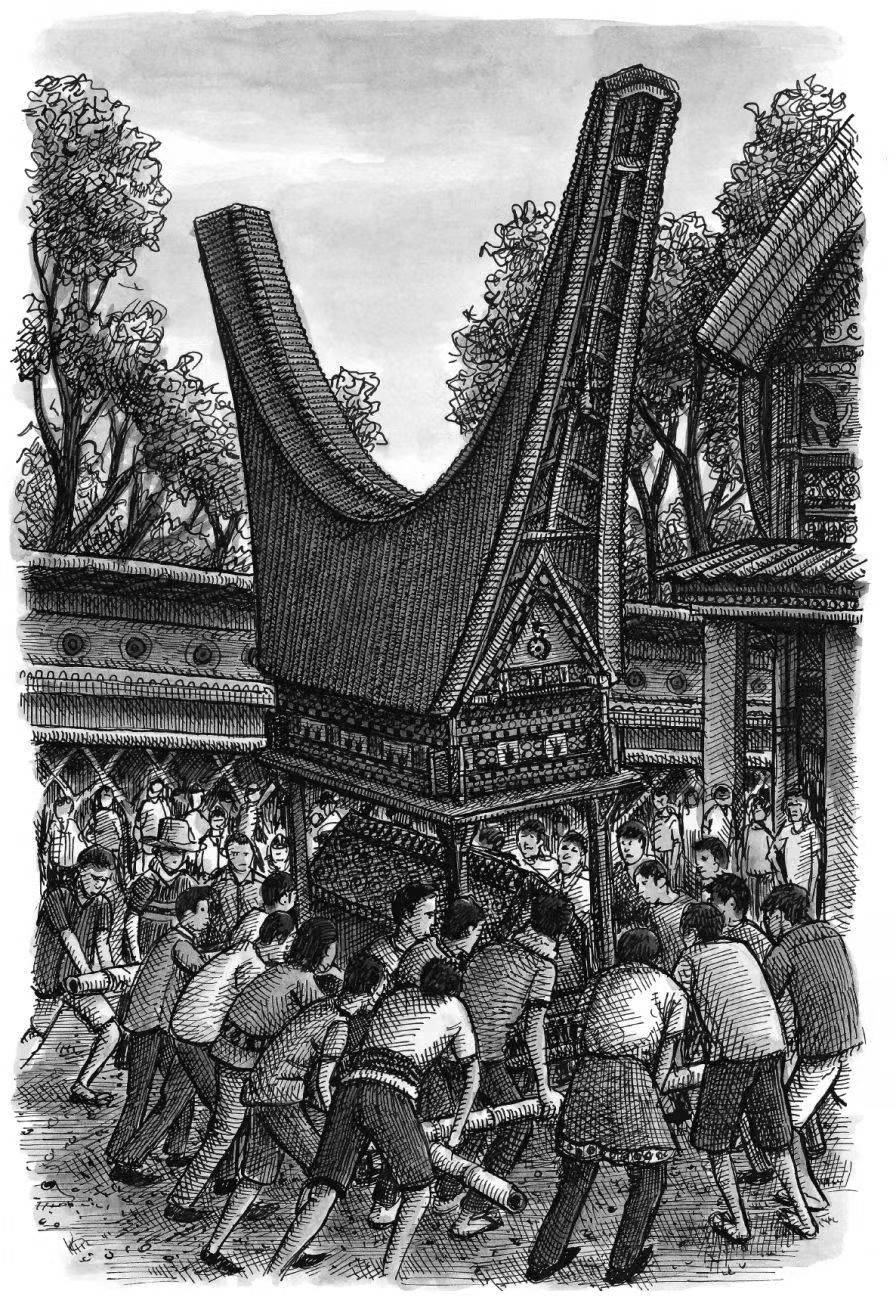
\includegraphics[width=\linewidth ,totalheight=0.95\textheight , keepaspectratio]{塔纳托拉雅的葬礼.jpg}
\caption{塔纳托拉雅的葬礼}
\label{fig:ta_na_tuo_la_ya_de_zang_li}
\end{figure}

人们一拥而入进了院子中央,而抬棺的队伍此时还在外面缓慢前进着。棺房比想象的要沉,小伙子们只能每走半分钟就把它放下来休息。

院子中央有一头强壮的水牛,它神情凝重,仿佛已经猜测到了自己的结局。它被一根短绳子拴在旁边的木桩上,可怜的模样...

游客(我猜的,他们有几个人皮肤白皙,带着西欧口音)统一集中在院子远处的角落里,所在之处和主场地隔着一排栅栏。这个措施反映出塔纳托拉雅死亡旅游业的一个棘手问题:如何才能既让游客近距离参观,又不让他们离得太近。我们也在这个“看台后排区”,但我不觉得有什么不妥。我找好地方坐下,保罗拿出相机准备拍照。为了让自己在闷热潮湿的天气里好过点儿,保罗今天换了一身行头:一件牛仔上衣、一条牛仔工装裤、一个警长徽章、一双波点短袜和一顶牛仔帽。

有些游客不太明白“后排区”的意义。一对夫妇直接坐进了留给死者家属的贵宾区。但当地人太客气了,没好意思把他们赶走。一个染着扎眼金发的德国老太太径直走到院子中央,用iPad对着小孩的脸就是一顿猛拍,还一支接一支地抽着红色万宝路烟。我真想找根拐杖钩着她的脖子把她弄走。

塔纳托拉雅的旅游业在最近几十年才兴起,20世纪70年代之前几乎没有人听说过这个地方。当时,印度尼西亚政府重点开发巴厘岛和爪哇岛的旅游业(事实证明他们做得很成功),忽视了塔纳托拉雅的独到之处——观赏性和仪式性兼具的传统葬礼。塔纳托拉雅不想再被其他印度尼西亚人看作“割取别人首级进行黑巫术”的地方,而是希望以保存良好的传统文化而闻名。

遗体终于被抬进了院子。抬棺人将棺房举起再放下,如此反复,口中哼着歌谣。他们一刻不停,直到全身的力气用尽之后才把棺房放到地上。他们喘了几口粗气,接着又把棺房扛在肩上,重复之前的动作。这种力量的交替让我看得入迷,西式葬礼的抬棺仪式一下子就显得有些古板。

这具遗体生前属于罗文纳斯·林汀。他是一位政府公职人员,也是一个农民,是村里的重要人物。我身后就放着一张5英尺高的照片,上面是林汀先生的脸部特写。照片里的人大概60岁,留着细长胡须,穿着时髦的蓝色西装。

身穿特色串珠服饰的小孩子在院子里追逐打闹,不时给搬运活猪的人让路。这些猪绑在竹板上,不断地发出尖锐的叫声。几个人把猪抬到屋后宾客看不见的地方。主屋的大门前挂着一个门帘,上面画满了迪士尼公主。在贝儿公主、爱丽儿公主和爱洛公主的注视下,这些猪穿过了通向屠宰场的大门。不知道我们早些时候碰见的黑毛猪是否也在其中。

塔纳托拉雅的葬礼可不是普通的自带酒水型(这里的“水”是水牛的“水”)活动。每一只献祭的动物都来自不同的人家,而且有记录可查。因为这套份子体系,人们通常不会错过别人的葬礼。就像阿古斯说的:“你在我妈妈的葬礼上送来一头猪,那我也要在你家举行葬礼时还一头。”看来,塔纳托拉雅式葬礼和美国葬礼一样,也存在过度花费的问题,因为不愿意被人看作不尊重死者。

到目前为止,这场葬礼上的仪式看上去都很繁复\footnote{繁多复杂。},但阿古斯说这已经比从前简单多了。阿古斯的父母从出生起就信奉阿鲁克教,但父亲在16岁时皈依了天主教。对此,阿古斯的解释是:“阿鲁克教里有7777种仪式,这太复杂了,人们只好改信别的。”我可不觉得天主教的仪式少,但就这样吧。

当牧师走到麦克风前开始布道时,人们安静下来。我听不懂他在讲什么,但能听出有几次他停下来,大声呼喊死者的名字向其致意:“罗——文纳斯,林——汀——!”他连续不停地讲了20多分钟,内容大多是重复的。很多人都准备离场,这时他贴近麦克风大吼了一声:“CO——E——!”那个动静活像是死亡金属乐队的主唱发出来的。告诉你,如果你恰好坐在音箱边上,却没在“CO——E——!”这个词出现时及时逃开,后果一定惨不忍睹。阿古斯告诉我,“COE”类似“好好听着”。据说,塔纳托拉雅的葬礼悼词在近几年深受电视节目的影响(舞蹈风格和服装设计也是)。

按照西方医学对死亡的定义,罗文纳斯于5月底去世,也就是葬礼前3个月。但按照塔纳托拉雅的习俗,他其实还活着。虽然已经没有了呼吸,但塔纳托拉雅人认为他只是处于类似发烧这样的生病状态。这个状态会一直持续到人们献上第一个活祭,通常是一头水牛或一头猪。献祭之后,罗文纳斯就可以ma’karu’dusan(咽下最后一口气),和作为祭品的动物一起死去。

人类学家迪米特里·辛吉罗尼斯在塔纳托拉雅进行了两年的田野研究,其间和一位名叫奈拉雅的当地老人建立了深厚的友谊,老人把迪米特里看作亲儿子一般。9年之后,迪米特里重返塔纳托拉雅,本以为能给奈拉雅一个惊喜,没想到她已经在两周前去世了。迪米特里来到奈拉雅家,她的一个亲戚把他领到后屋,然后告诉奈拉雅,迪米特里“回来了”。

\begin{quotation}
我端详着她的脸,然后盘腿坐下,在她耳边轻声问好。虽然一侧脸有腐烂、脱落的迹象,但她看上去十分宁静、安详……她只是“睡着”(mamma’)了,但她“知道”(natandai)我来看她了。不仅如此,她听得到也看得见我。她没有“死”(mate),只是“生病”(hot)了。因此,她还是“能够感受到一切”(nasa’dinganapa-apa)。
\end{quotation}

按照塔纳托拉雅的习俗,遗体在葬礼之前要放在家中。这听上去好像没那么震撼,但让我告诉你,在家中这段时间少则几个月,多则好几年。在此期间,死者的家人负责把遗体制成木乃伊,还要给他送饭、换洗衣物,时不时还要跟他说说话。









保罗第一次来塔纳托拉雅时,问阿古斯是否觉得家里待着一个已经死掉的亲戚很恐怖。阿古斯听了后放声大笑:“我小时候,我爷爷的遗体在我家待了7年。我跟我哥哥,我俩和他睡在同一张床上。每天早上,我们都给爷爷穿好衣服,然后把他靠墙立着,晚上睡觉时再把他放回床上。”
根据自己的所见所闻,保罗认为在塔纳托拉雅,死亡并不是一道强行把生者和死者隔开的“难以逾越的鸿沟”,而是一个模糊的界限。塔纳托拉雅人万物有灵的信仰也强调人类和非人类,不管是动物、高山还是尸体,两者之间都没有绝对的隔阂。


根据自己的所见所闻,保罗认为在塔纳托拉雅,死亡并不是一道强行把生者和死者隔开的“难以逾越的鸿沟”,而是一个模糊的界限。塔纳托拉雅人万物有灵的信仰也强调人类和非人类,不管是动物、高山还是尸体,两者之间都没有绝对的隔阂。
牧师总算讲完了,最后一嗓子“好好听着”也逐渐从音箱中消失。保罗轻轻走到我身边,低声说:“他们杀死那头牛后,应该顺手把某些游客也解决了。”
这时,两名男子好像收到信号一般,同时向院子里的水牛走去。一个人把一根蓝色的绳子从牛的鼻环中穿过。他的动作很轻柔,一边操作,一边用手挠着牛的下巴。水牛貌似没有意识到自己成了全场的焦点。另一个人蹲下来,把它的两只前蹄拴在地上的木桩上。
我不确定自己还在等待什么,也许是一段吟唱,也许是死者家属的相聚?这时,第一个人牵起牛头,从腰带里抽出一把砍刀瞬间割开了牛的喉咙,整个过程只有几秒钟。水牛向后仰起身躯,健壮的肌肉和牛角清晰可见。它想逃跑,却被绳子牢牢地固定在原地。一道鲜红的刀口出现在它的喉咙上,但没有血流出来,看来刀口不深。
好几个人冲上前拽住牛鼻环上的绳子,但没能制服它。水牛又踢又踹,猛烈地摆动自己的身躯,喉咙上的伤口撕裂开来,暴露在众人面前,这个场面让人难以直视。一个人拿出砍刀,朝牛脖子再次砍了下去。这一次,鲜血瞬间喷溅出来。
水牛发疯似的腾空跳起,力量大到挣脱了绳子和木桩的束缚,跌跌撞撞地冲向右侧的人群。现场一片混乱,尖叫声此起彼伏。我用小型摄像机拍下的视频也因此进入《科洛弗档案》(5)模式,记录下来的全是沉重的呼吸声和踩踏地面的闷响。我周围挤满了慌张的人,推搡之中,我不小心割破了手。
[插图]
当时,我确信会有人(很可能是我自己)死于水牛的报复行动。最后,司仪成功把牛抓回了院子中央。不久之后,水牛倒地死去,喉咙上的伤口汩汩地往外冒着血。人群中有人哭有人笑,两种截然不同的声音混合成一种缤纷的复调。刚才的惊心动魄向葬礼注入了一丝活力。


阿古斯正在打电话,语气很激动。
“出什么事儿了?”我问保罗。
“我们得带头猪过去。”
“我们去哪儿找猪啊?”
“阿古斯说他可以帮忙。不带头猪过去不礼貌。”
阿古斯的车已经坐满了,里面有我、保罗、阿古斯、司机和阿托——一个搭顺风车去隔壁村庄的15岁少年。车上已经没地方放猪了。
阿古斯挂断电话,向我们宣布道:“明天,我的一个朋友会骑摩托车把猪送来。”
阿托一路上都在疯狂地发短信。和一群成年人挤在一辆车里,换作哪个青少年都会这样吧。阿托家将在马聂聂节上给他叔叔和曾祖父开棺,这两个人在阿托还没出生的时候就去世了,因此阿托只能和他们的遗体相逢。
我们到达了目的地。这是一个由多个独立小村庄组成的村镇,没有所谓的中心。大部分村民都以种植水稻为生,包括我们此行的东道主。他们几户人家住在传统的长屋里,一共七栋,中间是公共生活用的庭院。院子里,一群红冠大公鸡正被几只瘦骨嶙峋的狗追着跑,边跑边“喔喔”地叫,狗后面还跟着几个笑哈哈的小孩。女人们正在用细长的竹竿敲打刚收获的稻谷,动作一刻不停。
村子里陆陆续续来了不少人,他们开始帮忙清理房子状的墓室。村子现在共有十几个墓室,都在自家屋子附近。每个墓室的门上都挂着一把大锁,这在以前是没有的。这么做不是为了提防邻居,而是因为几年前有人从村里偷走一具干尸,卖给了兰特包的一个收藏家。后来,村民打听到了是哪个收藏家,又去人家那里把干尸偷了回来。


几个人正聚在一起讨论如何给墓室通风。两年前,村里安葬了一个名叫约翰·汉斯·塔皮的村民。现在,他的深色木质棺材翘开了一个角,一打开墓室的大门就能看见。塔皮的儿子担心墓室里的空气过于潮湿:“希望父亲没什么事。但愿他还是干燥的,没有腐烂。”
今年的马聂聂节对约翰·汉斯·塔皮可谓意义重大。他的儿子认为,父亲在两年前去世时,家里在物质方面做得不够好——当时家里穷,没有杀牛献祭。他对此一直耿耿于怀,坚信没有活祭的话,“父亲就不能转世再生了”。不过,这一切将在这周改变:献祭的水牛已经选好了,正拴在附近的空地上呢。
两个墓室已经打扫完毕。一个女人敞开墓室的门,拿着一大罐柠檬味清新剂往里喷。
路的尽头有一户人家刚刚宰完猪,正等着新教牧师前来给他们新建的、能装下六个家庭成员的墓室赐福。他们邀请我们共进晚餐。
切成块的猪肉盛放在竹盘里,正架在火上烧烤。猪是在炉子旁边杀掉的,现在我们就坐在干掉的猪血旁吃晚饭,几只苍蝇绕着我们飞来飞去。不远处的竹架上挂着几只猪蹄。一只小狗冲进来,叼起一块滴着血的猪下水就往外跑。“哎哟!”厨子冲小狗大叫了一声,但没有阻止它带走战利品。
一个女人递给我一片竹叶,上面放了一个热乎的粉色饭团。这时,有人把竹盘上的肉从火上取下来,一大堆肥肉烧得滋滋作响。吃到一半时,我把这盘肉拿到跟前仔细瞧了瞧:焦脆的脂肪表皮上,一个个毛囊清晰可见。这可是动物尸体上的一块肉啊,我突然反应过来,随即感到一阵厌恶。
我虽然在人类遗体上花了很多时间,但不熟悉动物尸体,不是包装在保鲜膜和塑料泡沫盒里的动物我就不认识。法国人类学家努艾莉·维亚莱斯的一篇关于法国食物体系的文章中有一段话,我觉得也适用于西方其他国家:“屠宰被认为应该是工业化的,即大型化、统一化。不能存在暴力(最好是无痛的),也不能被人看见(最好根本不存在)。这几点即使做不到也要做到。”


即使做不到也要做到。
饭桌上有一位老奶奶,年龄大到眼睛里蒙上了一层白膜。她拿起一小撮米饭,看向屋外山谷的方向。她不怎么与坐在旁边的人交流,也许她已经说不动话了。阿古斯用沾满猪肉残渍的手指捅了我一下,然后悄声说道:“那个新墓穴应该就是给她准备的。”阿古斯在调侃她,但说的也算是事实。这位老奶奶很快就会踏上祖先走过的路,搬到她的新房子里,那个“没有火也没有炊烟的房子”。
夜里,我们的猪乘着摩托车到了。它一着地就钻进其中一栋木屋,狼吞虎咽地吃着泔水。它完全没有意识到,因为我和保罗,这里将成为它的葬身之地。
这天晚上,我们都住在长屋里。长屋从外面看上去很宽敞,但我们进屋爬上梯子后却惊讶地发现,楼上只有一个没窗户的单人间。好在房间的地板上已经铺好了被褥,我们躺下后很快就睡着了。后半夜时,我们才意识到这里不是单人间,墙壁上的木闩拆下后,推开就可以看到另外三间屋子。一整晚都有人蹑手蹑脚地在我们房间周围进进出出。
* * *
第二天一早,一阵阵凄凉的铜锣声从路边传来,正式宣告马聂聂节拉开帷幕。
我见到的第一具木乃伊戴了一副20世纪80年代的飞行员墨镜,镜框还镶着金边。
“哎哟,”我心想,“这哥们儿跟我中学的代数老师一个风格。”

一个年轻人把这具干尸立起来,另一个人拿起剪刀,把他身上的蓝色上衣从领口一路向下剪开,直到露出内裤边缘。木乃伊的上身和双臂就这样暴露在空气中。这个人虽然已经死去八年,但遗体保存得非常完好,表面上没有肉眼可见的伤口或裂痕。跟他隔着两具棺材的哥们儿就没那么走运了:全身上下都皱巴巴的,只有一层薄薄的干皮勉强搭在骨头上,要不是裹了一条镶有金边的毯子,估计早就散架了。
刚才那具木乃伊被放在地上,头下垫了个枕头,身上只剩下平角短裤和飞行员墨镜。一张8英寸×10英寸(6)的遗像照片摆在它身旁。照片上的他看上去一点儿也不像我的代数老师,人在八年间的变化还真大。
[插图]
几个女人在他旁边跪下,一边轻抚他的脸颊,一边大声哭着呼唤他的名字。当哭喊声逐渐停下时,他的儿子手捧一套工具刷(就是五金店里卖的那种)走了过来,开始清洁遗体。他用刷子轻轻扫过父亲粗糙的皮肤,每一下都很利落,并且充满爱意。一只蟑螂从父亲的平角短裤里蹿了出来,但他好像并不在意,继续手里的动作。这种打理遗体的方式我还是第一次见。


10分钟前,阿古斯接到一个电话,对方说有一家人正在河边一处难以到达的墓室中给死者开棺。我们迅速沿着水稻田旁的土路朝那个方向跑去。路的尽头是一条棕黄色的泥沟,附近没有垫脚的石头,也没有桥。我们只好一边抱怨,一边从泥里蹚过去,其间我还摔了个屁股蹲儿。
到达目的地后,我们看到至少有40具遗体被抬了出来,在地上一字排开。有些遗体裹着颜色鲜艳的布料,有的放在狭长的木质棺材里,还有的用印满卡通图案——凯蒂猫、海绵宝宝,以及一大堆迪士尼卡通人物——的毯子包着。这家人在遗体间走来走去,商议要先给谁开棺。有些死者他们已经不记得是谁了,有的则是重点关照的对象,比如某人亲爱的丈夫或某家的宝贝女儿,他们的家人都迫不及待地想再见到他们。
一个母亲正在打开16岁儿子的棺材。最先露出来的是一双弯曲变形的小脚,然后是手,看上去保存良好。站在棺材两侧的人试着抬起男孩,他们动作轻柔,确保不会碰坏遗体。他们成功地把男孩立了起来。男孩的躯干完好无损,但头部已经白骨化了:牙齿清晰可见,浓密的黑发还连在头皮上。但他的母亲毫不介意,此刻正欣喜若狂地看着他。这份喜悦也许是一时的,也许她从来都是这样,但不管如何,现在她正握住他的手,轻抚着他的面庞。
附近有一个人在用刷子清洁父亲的遗体。父亲的脸被蜡染布料制成的裹尸布染成了粉红色。“他是个好人,”他说道,“他有八个儿女,但他从没打过我们。我很难过,但又很开心,因为我现在能照顾他了,就像他以前照顾我那样。”
塔纳托拉雅人会把自己接下来的动作讲给遗体听:“现在,我要把你从坟墓里移出来。”“抱歉只给你买了烟,我最近手头有点儿紧。”“现在,我要脱掉你的外衣。”“你女儿和女婿从望加锡过来看你了。”
我们在这个河边墓穴碰到了这家的族长,他对我们的到来和送上的香烟表示感谢。他允许保罗拍照,也同意我问问题,但条件是答应他的一个请求:“如果你们在村子里碰见外来人,不要告诉他们这个地方,这里是我们的秘密。”
我想起前几天葬礼上那个粗鲁的德国女人,一边抽烟,一边把iPad贴在别人脸上乱拍。我担心自己也变得跟她一样——我们渴望把期待已久的事物看个遍,但不承想这让我们变成了不受欢迎的人。


我们穿过稻田返回主路,正好赶上东道主开棺打理自己家的遗体。我认出一个在兰特包当平面设计师的同龄人。昨天深夜,他骑摩托车赶了回来,在我们睡觉的房间钻进钻出。他指着一具包在金色布料里的骷髅说道:“这是我兄弟,17岁时骑摩托车出车祸死了。”然后指了指旁边的遗体,“那是我爷爷。”
我们下方的山坡上有一家人在野餐。用餐完毕后,他们把死去七年的祖父平放在方格桌布上。这是他祖父第二次参加马聂聂节,遗体状态极佳,看不出有任何损坏。这家人先用软刷清洁他的面部,再把他翻过来清理脑后干裂开的皮肉。拍摄全家福时,祖父被立在中间,家庭成员纷纷围过来,有的表情严肃,有的面带笑容。我正津津有味地看着,一个女人招呼我过去一起合影。我朝她摆摆手,意思是“还是不用了吧”,但他们坚持要叫上我。于是,一张奇特的合影出现在印度尼西亚的深山里,上面是我、一个塔纳托拉雅家庭和一具焕然一新的干尸。
[插图]
我之前听说把遗体制成木乃伊通常发生在气候寒冷干燥的地区,没想到在湿润多雨的印度尼西亚也能这么做。那么问题来了:这里的遗体究竟是怎么变成干尸的呢?不同的人会给你不同的答案。有人说他们用的是自古流传下来的方法——把油灌入死者的嘴巴和喉咙里,再用特制的茶叶和树皮覆盖全身。茶叶的茶多酚和树皮将皮肤中的蛋白质收紧,从而强化了皮肤的柔韧性和硬度,这样就能够更有效地抵挡细菌入侵。这个过程与标本师对兽皮进行处理使之长久保存的过程类似(所以有一种皮革叫“植鞣皮”)。
塔纳托拉雅现在还流行一种新潮的干尸制作方式:把防腐师的好朋友福尔马林注射到遗体中。有一个女人告诉我她无法接受这种方式,因为不愿意死去的家人被针扎。“但我知道有人这么做。”她压低声音说,好像发现了什么见不得人的事。


生活在塔纳托拉雅这部分的村民可以称得上业余人体标本师了。既然他们现在和北美人民都用同一种化学制剂给尸体防腐,我不明白为什么西方人依然会被他们的习俗吓个半死。原因应该和尸体干燥的程度无关,而在于塔纳托拉雅人不把遗体密封在棺材里,也不把棺材搁置在水泥做成的地下墓穴里,而是大大方方地让遗体和活人待在一起。(7)
一听到母亲的遗体在家里放了七年,许多西方人立刻就会联想到电影《惊魂记》及其主人公——精神失常的酒店经理诺曼·贝茨。塔纳托拉雅人保存母亲的遗体,诺曼·贝茨也保存母亲的遗体;塔纳托拉雅人和家人的遗体生活了很多年,诺曼·贝茨也和母亲的遗体生活了很多年;塔纳托拉雅人像对待活人似的跟死者交谈,诺曼·贝茨也像对待活人似的跟妈妈的遗体交谈。但是,塔纳托拉雅人可以稀松平常地用一个下午的时间清洁遗体,诺曼·贝茨却被美国电影学院选为影史上最可怕的反派角色第二名,名列汉尼拔·莱克特和达斯·维德(8)之间。他的排名之高,并不是因为装扮成已故母亲的模样对无辜的房客痛下杀手,而是因为西方人觉得他长期和遗体进行互动的行为过于吓人(好像严重剧透了,抱歉)。
[插图]
昨天,我碰到了约翰·汉斯·塔皮的儿子,今天我要去见约翰·汉斯·塔皮本人。他被平放在地上晒太阳,身上只穿了一条平角裤,手腕上戴了一块金表。他的胸腔和腹腔注满了福尔马林,因此这两处保存得异常完好。相比之下,他的面孔已经变成黑色,上面布满了斑点,白色的骨骼依稀可见。这时,他的家人把刷子伸到他的平角裤里,开始清洁他那干瘪的阴茎。不出意料,家人的脸上写满了尴尬。他们互相开了个玩笑,然后继续手里的活儿。
小孩子们在木乃伊之间跑来跑去,他们有时会在某具遗体面前突然停下,仔细瞧一瞧之后再伸手捅一下,然后大叫着跑开。一个5岁的女孩爬了上来,和我一起坐在一个墓室的屋顶上看着他们玩闹。我俩没有说话,心照不宣地享受着俯视他人的奇妙快感。


阿古斯发现我在屋顶上,向我喊道:“喂,我在想我之后是不是也会变成这样。肯定会的,是吧?”
我们回到留宿的那栋房屋后,一个4岁的男孩过来偷看我们吃饭。他从篱笆后面探出头,每次我回头冲他做鬼脸时,他都开心地大叫。这时,他妈妈过来告诉他不要打扰我们,于是他给自己找了个小刷子。他穿过院子走到一堆干竹叶旁坐下,用刷子全神贯注地在地上刷来刷去,保证每一条小裂缝都被刷到。如果马聂聂节一直存在,长大成人的他也一定会去清洁某具遗体,遗体的主人说不定就是我们这次碰见的某个村里人。
* * *
第二天清晨,约翰·汉斯·塔皮已经换上了一套新衣服,上衣是一件装饰着金色纽扣的黑夹克,下装是一条海军蓝休闲裤。他今天要被搬去路尽头的一间新墓室里,墓室的墙壁是浅蓝色的,屋顶上立着一个白色十字架。里面的装饰走的是多元文化路线:除了传统的水牛符号之外,还有玛利亚之心、耶稣祈祷像以及《最后的晚餐》全景图。
家里人把约翰立起来,跟穿着新衣的他拍了最后一张合影,便把他放回棺材。他们把闪亮的黑皮鞋从他脚上脱下放在旁边,给他裹好毯子,随后合上了棺材盖。棺材两侧被擦拭干净之后,他们就把棺材扛在肩上出发了。鼓声和诵经的声音伴随了他们一路。
我往车上装东西时,阿古斯走了过来。“知道吗,现在就有具尸体在这栋房子里。”他指着跟我们木屋只隔了10英尺的一栋传统房屋说道。一位名叫山达的70岁老太太两周前死在这栋房子里。这家人一直瞒着我们,就是想看看我们知道后会有什么反应。
“你想见见她吗?”阿古斯问道。
我慢慢地点了点头。不知为什么,我觉得我们应该就睡在尸体隔壁。


“嘿,保罗,”我叫醒正在屋里补觉的保罗,“跟我下楼,给你看样东西。”
在阿古斯的指导下,我们给山达带来了一些吃剩的食物——她应该知道是我们送的。我们钻进里屋,看到山达躺在一张竹席上,身上盖着一条绿色的格纹毯子。她穿着一件橘色的衬衫,脖子上围了一条粉色的围巾,身边还放着钱包和食物。她的脸上围着一块布,面部皮肤有着橡胶般的质感,这在防腐后的遗体上很常见。
山达是由一个本地的专业人员用福尔马林防腐的。她的家人没有亲自操作,因为觉得福尔马林太“辣眼睛”。山达一家子都是成功的稻农,没有时间按照传统天天照料她的遗体。
她会在家里一直住到搬进墓室。这期间,家人给她端茶倒水,她在梦里与家人相会。距离她穿过生与死那条模糊的界限只有两周,因此家里人决定,等味道散去后就跟她一起睡。
阿古斯小时候跟他祖父的遗体睡了七年。他耸了耸肩,说道:“这种事情我们已经习惯了,这就是生与死。”
* * *
在前往印度尼西亚之前,我试图在网上查询与塔纳托拉雅有关的信息,想先看看会有什么样的丧葬仪式在等着我。搜索出来的信息很少,起码没什么英语的(你在谷歌搜“ma’nene’”,出来的结果是《亚特兰大娇妻》的主演宁宁·利克斯)。
照片也没有几张,其中最清晰的一张来自英国报纸《每日邮报》。我不知道他们是从哪儿得到的这张照片,因为他们显然没有派记者去。页面上的评论区很有意思,一条评论写道:“天哪,他们对这些逝者做了些什么呀?”另一条评论则写着:“讲真,这是对死者的大不敬。”
确实,如果说把莎莉姨妈从明尼苏达的坟里挖出来,把她放到高尔夫球车上在郊区民宅附近转一圈儿,那么是的,这的确是对死者的大不敬。但这些心智不健全的网友没有意识到,人死后,亲情还会继续存在。塔纳托拉雅人不但不觉得开棺掘尸是对死者的不尊重(事实上,这是对死者最大的尊重),而且认为这是与逝去的家人维持情感的一种方式。
作为一名殡仪业者,我总会碰到各种各样关于母亲遗体的问题。你不知道我听到了多少次:“我妈妈11年前在纽约州北部去世,防腐后葬在我们的家庭墓地里,你能告诉我她现在变成什么样了吗?”这个问题的答案取决于多个因素:天气、土壤、棺材、化学品。所以,我给不出一个完美答案。当我看到塔纳托拉雅人与母亲的遗体互动时,我意识到他们不需要通过殡仪人员了解遗体的状况。他们很清楚自己的母亲死后是什么样子,哪怕她已经死了11年。相较于与死去的母亲重逢,还是人类的胡思乱想更可怕一些。


\hr 


\part{附录}
\chapter{术语释义}
\section{世纪的早期中期和晚期}
表达时间不需要太过于精确的时候,会将一个世纪分为三个不同的时期来表达。一个世纪约一百年,前三十年称之为早期,中间四十年称之为中期,后三十年称之为晚期。

\section{非公制单位}
1码约0.914米

1磅约0.454千克

1加仑约4.546升

1立方英尺约0.028立方米

1英尺约0.3048米

\chapter{参考资料}
\begin{itemize}
\item 1
\end{itemize}

% 编者:Wander
\end{document}


